% IEEE Transactions on Wireless Communications (TWC) submission.
% Initial submission limit: 13 double-column single-spaced pages (10 pt).
\documentclass[journal,10pt]{IEEEtran}

\usepackage{cite}
\usepackage{amsmath,amssymb,amsfonts}
\newtheorem{proposition}{Proposition}
\usepackage{algorithmic}
\usepackage{algorithm}
% Unnumbered full-width header line inside algorithmic (for phase markers).
% Empty-label \item skips both the line number and the ALC@line counter,
% while inheriting the current block indent.
\makeatletter
\newcommand{\PHASE}[1]{\item[]{\normalfont\bfseries #1}}
\makeatother
% STA-count notation: visitor / native populations
\newcommand{\Nvis}{N_\mathrm{vis}}
\newcommand{\Nnat}{N_\mathrm{nat}}
\usepackage{graphicx}
\usepackage{array}
\usepackage{subcaption}
\usepackage{textcomp}
\usepackage{url}
\usepackage{xcolor}
\usepackage{stfloats}

% TWC: figures and tables are placed with the text, not collected at the end.
\renewcommand{\topfraction}{0.9}
\renewcommand{\bottomfraction}{0.8}
\renewcommand{\textfraction}{0.07}
\renewcommand{\floatpagefraction}{0.8}
\setcounter{topnumber}{2}
\setcounter{totalnumber}{3}

\begin{document}

\title{PACE: Probabilistic Adaptive Contention Control for Non-Primary Channel Access in IEEE 802.11bn}

\author{Taewon Song and Yeunwoong Kyung
% \IEEEauthorblockA{\textit{Division of Electronics and Electrical Engineering} \\
% \textit{Dongguk University}\\
% Seoul, Republic of Korea \\
% twsong@dongguk.edu}%

\thanks{T. Song is with the Division of Electronics and Electrical Engineering, College of Engineering, Dongguk University, 30, Pildong-ro 1-gil, Jung-gu, Seoul 04620, Republic of Korea (e-mail: twsong@dongguk.edu) and Y. Kyung is with the Department of Electronic Engineering, Seoul National University of Science and Technology,
Korea. (e-mail: ywkyung@seoultech.ac.kr), Corresponding author: Y. Kyung}%

\thanks{This work was supported in part by the National Research Foundation of Korea (NRF) grant funded by the Korea government (MSIT) (No. RS-2026-25481311), in part by Institute of Information \& Communications Technology Planning \& Evaluation (IITP) grant funded by the Korea government (MSIT) (No. RS-2026-25523610), and in part by the Dongguk University Research Fund of 2026.}
}

\maketitle

\begin{abstract}
While an overlapping basic service set (OBSS) transmission occupies the primary channel, adjacent non-primary channels sit idle because conventional IEEE 802.11 mandates that the primary channel be included in every access. IEEE 802.11bn introduces non-primary channel access (NPCA) to exploit these idle intervals. The standard contention mechanism, however, is ill-suited to NPCA's constrained transmission windows, as its collision-triggered backoff growth synchronizes stations into repeated collisions or pushes their counters beyond the remaining opportunity, wasting airtime that could carry data.
We propose PACE, a probabilistic adaptive contention control scheme that lets stations track the time-varying fair-share transmission probability of the depleting window without central coordination. PACE combines a deadline-scaled initialization and a distributed multiplicative feedback rule that copies the successful sender's probability on solo receptions, together with a proactive self-exclusion mechanism that silences stations whose frame length exceeds the remaining window.
We evaluate PACE under IEEE 802.11 standard timing on a non-primary channel shared with native stations, against the standard-compliant NPCA baseline and a genie-aided fair-share reference. Across $5$--$50$ visiting stations, PACE keeps the total useful airtime within $3\%$ of the fair-share reference under request-to-send/clear-to-send (RTS/CTS)-protected access, up to $61\%$ above the standard procedure and up to $4.1\times$ under basic access, while holding the visitors' airtime at or below their population-proportional share. The advantage grows with the visitor population, where standard backoff idles behind frozen counters and collides in synchronized bursts.
These results establish probabilistic, deadline-aware contention as a design reference for non-primary channel access in next-generation Wi-Fi.
\end{abstract}


\begin{IEEEkeywords}
Non-Primary Channel Access, IEEE 802.11bn, Probabilistic Access Control, OBSS, Adaptive Contention, Wi-Fi
\end{IEEEkeywords}

\IEEEpeerreviewmaketitle

% Introduction
\section{Introduction}
\label{sec:introduction}

Spectrum efficiency in next-generation Wi-Fi networks depends critically on how effectively stations (STAs) exploit available channel time. In dense deployments, overlapping basic service sets (OBSSs) routinely occupy the primary channel while adjacent channels remain idle, creating a persistent underutilization problem. Hence, IEEE 802.11bn addresses this gap by introducing non-primary channel access (NPCA), which allows STAs to transmit opportunistically on non-primary channels during ongoing OBSS intervals~\cite{ieee80211bn,wei2024non}.

NPCA, however, presents a contention challenge distinct from conventional channel access. Each opportunity lasts only as long as the ongoing OBSS transmission, so competing STAs must resolve their access within a finite, depleting window. To govern this access, the IEEE 802.11bn draft has STAs on the non-primary channel reuse the same binary exponential backoff (BEB) mechanism that the distributed coordination function (DCF) employs on the primary channel~\cite{ieee80211bn}, yet BEB was designed for open-ended contention. On the primary channel, doubling the backoff window after each collision harmlessly spreads out retransmissions; within a bounded NPCA window the same growth turns harmful, as the inflated backoff frequently exceeds the time remaining. STAs whose counters overshoot the deadline are silenced for the rest of the interval, leaving the channel idle even when they still have data to send. Heterogeneous frame lengths compound the problem, since the draft leaves unspecified what a STA should do when its frame no longer fits the remaining window; a compliant STA may keep contending, or transmit only to be cut off at timer expiry, despite having no viable transmission opportunity.

% Consider a dense office environment where multiple STAs detect an OBSS transmission
% and attempt to use the secondary channel concurrently. Early collisions trigger
% exponential backoff growth; within a few rounds, a large fraction of STAs have
% accumulated backoff counts that exceed the remaining window duration. The channel
% spends the final slots idle, not because no STA wanted to transmit, but because
% the contention mechanism pushed every backoff counter beyond the opportunity horizon.

Existing work on NPCA has focused on characterizing aggregate throughput and delay under the standard switching rule, taking BEB within the non-primary channel as given \cite{wei2024non,bellalta2025performance,wei2024optimized}. The contention dynamics within the finite NPCA window, and the mismatch between BEB's infinite-horizon design and the window's bounded duration, have not been addressed. Adaptive probabilistic schemes, in turn, are built for infinite-horizon operation and converge to a static equilibrium, so they too fail to track the optimal access probability as the window shrinks and the set of viable STAs changes.

In this paper, we propose PACE, a probabilistic adaptive contention control scheme for NPCA that enables STAs to collectively track the time-varying fair-share transmission probability of each moment within the window, without central coordination or explicit inter-STA signaling. PACE adapts the multiplicative-increase and multiplicative-decrease (MIMD) feedback rule inspired by the probabilistic neighbor discovery (PND) algorithm \cite{song2014pnd} to the finite-window NPCA context. STAs copy the successful sender's probability on solo receptions, reduce on collision, and increase on idle slots, causing distributed dynamics to track the fair-share policy. PACE further adds a physical protocol data unit (PPDU)-aware self-exclusion rule that silences STAs whose frame length exceeds the remaining window, eliminating a class of futile contention attempts that BEB would otherwise sustain.

The design of PACE is motivated by two requirements that are unique to NPCA's bounded-window structure: 1) the fair-share transmission probability is time-varying and must track the depleting window rather than converge to a static equilibrium, and 2) STAs whose frame length exceeds the remaining window must proactively self-exclude to prevent futile contention that wastes viable slots. The main contributions of this paper are as follows.

\begin{itemize}
  \item We characterize the fair-share transmission probability for finite-window NPCA, showing that it must continuously track the remaining window duration and the number of still-viable competing STAs, a deadline-driven, rising target that neither BEB nor existing infinite-horizon adaptive schemes can follow, since the latter react to a changing contending population but never to a window that is running out.
  \item We propose PACE, a fully distributed algorithm that addresses both requirements simultaneously. A deadline-scaled initialization and MIMD feedback drive the transmission probability toward the time-varying target without inter-STA signaling or knowledge of the total STA count.
  \item Through simulation in IEEE~802.11 standard timing on a channel shared with native DCF stations, we demonstrate that PACE keeps the total useful airtime within $3\%$ of a genie-aided fair-share reference under request-to-send/clear-to-send (RTS/CTS)-protected access and up to $4.1\times$ above the standard-compliant baseline under basic access, holds the visitors' airtime at or below their population-proportional share, and attains a per-attempt success ratio close to three times the baseline's, matching the fair-share reference; an ablation study further shows that both the deadline-scaled initialization and the self-exclusion rule are necessary for these gains.
\end{itemize}


The remainder of this paper is organized as follows. Section~\ref{sec:related_work} reviews related work on NPCA and adaptive medium access control (MAC) protocols. Section~\ref{sec:system_model} presents the system model. Section~\ref{sec:pace_algorithm} describes the PACE algorithm and its theoretical foundation. Section~\ref{sec:performance_evaluation} presents simulation results, and Section~\ref{sec:conclusion} concludes the paper.

\section{Related Work}
\label{sec:related_work}

This section reviews the two lines of work on which PACE builds, namely
NPCA in IEEE~802.11bn and adaptive contention control in wireless LANs, and
closes by contrasting them with PACE.

\subsection{Non-Primary Channel Access in IEEE 802.11bn}

IEEE 802.11bn introduces NPCA as a core mechanism for exploiting idle
secondary channels during OBSS transmissions~\cite{ieee80211bn,galati2024will}.
Wei \textit{et al.}~\cite{wei2024non} extended Bianchi's DCF model to a
multi-channel setting, establishing analytically that NPCA always outperforms
the non-NPCA mode; a follow-up study~\cite{wei2024optimized} incorporated
switching overhead and proposed a threshold policy to toggle between NPCA
and legacy modes based on primary channel occupancy. Bellalta
\textit{et al.}~\cite{bellalta2025performance} developed a Continuous-Time
Markov Chain model for a multi-BSS topology, identifying a secondary-channel
contention trade-off that can limit NPCA gains when the secondary channel
is shared. Lee and Song~\cite{lee2024impact} further showed that PPDU frame
duration has a nonlinear effect on inter-BSS coexistence, and Song~\cite{song2026adaptive}
applied deep reinforcement learning to the NPCA channel-activation decision.

Across these studies, however, efforts to improve NPCA performance target
the decision of when to switch to the non-primary channel, through
occupancy-based threshold policies~\cite{wei2024optimized} or learned
activation rules~\cite{song2026adaptive}, while the contention mechanism
exercised within the window is left fixed at BEB. How STAs should
adapt their access probability as the window depletes and viable STAs
drop out has not been studied.

\subsection{Adaptive Contention Control in Wireless LANs}

Bianchi~\cite{bianchi2000performance} established that BEB operates below
the theoretical throughput ceiling, and Cali \textit{et al.}~\cite{cali2002dynamic}
showed that p-persistent access can approach this limit in a distributed
manner, at the cost of estimating the number of active stations at run time
from the observed idle-slot statistics. Subsequent work has diversified
the adaptation mechanisms. BLADE~\cite{guo2026blade} uses a hybrid increase
multiplicative decrease (HIMD) policy
driven by a universally observable channel signal, although the target
access rate it regulates to is a fixed constant derived from a steady-state
throughput model; Wilhelmi
\textit{et al.}~\cite{wilhelmi2025s} impose structured transmission order
via inter-BSS activity awareness, which requires each STA to identify its
neighbors and maintain a list of them to derive its position in the order;
and learning-based approaches
optimize the contention window through deep Q-networks~\cite{zuo2025adaptive},
where the access point observes the collision rate and throughput of the
whole network, selects a contention window threshold, and hands it down to
its associated STAs in its beacons, or through fairness-constrained multi-agent policy
optimization~\cite{pan2025ai} trained centrally on the joint observations of
all agents.

Several of these schemes do follow a moving operating point, tracking a
target that shifts as the contending population changes. What none of them
represents is a deadline. All of them assume STAs contend over an
open-ended horizon, so their target never depends on how much time is left.
NPCA's bounded window demands a fundamentally different approach. The
optimal transmission probability must evolve as the window shrinks and the
viable STA population changes. The MIMD feedback rule of PND~\cite{song2014pnd} is
the closest mechanism in spirit, but was designed for infinite-horizon
neighbor discovery and provides no accounting for bounded window duration
or frame-length viability.

Table~\ref{tab:comparison} summarizes these distinctions along three axes.
\emph{Frame-fit self-exclusion} withdraws a STA whose frame no longer fits
the remaining window. A \emph{signaling-free} scheme transmits no control
information for its own sake, a value riding in a frame a STA sends anyway
not being counted, and $\triangle$ marks a scheme that adds no transmission
but must still infer the contending population from the activity of the
others. \emph{Time-varying target tracking} follows an operating point that
moves with the contending population rather than a static equilibrium. No
prior scheme withdraws an unfittable frame, and the schemes that do adapt
their operating point either track only the contending population or pay
for the adaptation with a view of that population, whereas PACE meets all
three requirements from purely local observations.

\begin{table*}[!t]
\centering
\caption{Comparison of contention control schemes.}
\label{tab:comparison}
\begin{tabular}{l >{\raggedright\arraybackslash}p{9cm} ccc}
\hline
\textbf{Method} & \textbf{Mechanism and objective} & \textbf{\shortstack{Frame-fit\\self-exclusion}} & \textbf{\shortstack{Signaling-\\free}} & \textbf{\shortstack{Time-varying\\target tracking}} \\
\hline
PND~\cite{song2014pnd}      & Multiplicative feedback with solo-copy rule; converge the transmission probability to the optimum without the contender count & $\times$   & \checkmark & \checkmark   \\
AND~\cite{vasudevan2013efficient} & Fixed-probability slotted ALOHA; discover all neighbors in finite time without coordination & $\times$   & \checkmark & $\times$   \\
Cali \textit{et al.}~\cite{cali2002dynamic} & p-persistent access with run-time estimation of the active station count; approach the theoretical throughput limit in a distributed manner & $\times$   & $\triangle$ & \checkmark   \\
BLADE~\cite{guo2026blade}   & Hybrid increase / multiplicative decrease toward a fixed target access rate; eliminate packet-delivery droughts for real-time Wi-Fi & $\times$   & \checkmark & $\times$   \\
IYT~\cite{wilhelmi2025s}    & Neighbor-ordered backoff interval assignment; reduce collision probability and worst-case latency & $\times$   & $\triangle$ & $\times$   \\
ACWB-DQN~\cite{zuo2025adaptive} & Deep Q-network contention window selection centralized at the AP; maximize throughput under varying network load & $\times$   & $\times$   & \checkmark   \\
FC-MAPPO~\cite{pan2025ai}   & Fairness-constrained multi-agent policy optimization; minimize collisions while ensuring inter-STA fairness & $\times$   & $\times$   & \checkmark   \\
\hline
\textbf{PACE (proposed)}     & \textbf{Multiplicative feedback with PPDU-aware self-exclusion; maximize channel utilization in the finite NPCA window} & \checkmark & \checkmark & \checkmark \\
\hline
\end{tabular}
\end{table*}

\section{System Model}
\label{sec:system_model}

\subsection{Network and Channel Model}
\label{subsec:network_model}

\begin{figure}
    \centering
    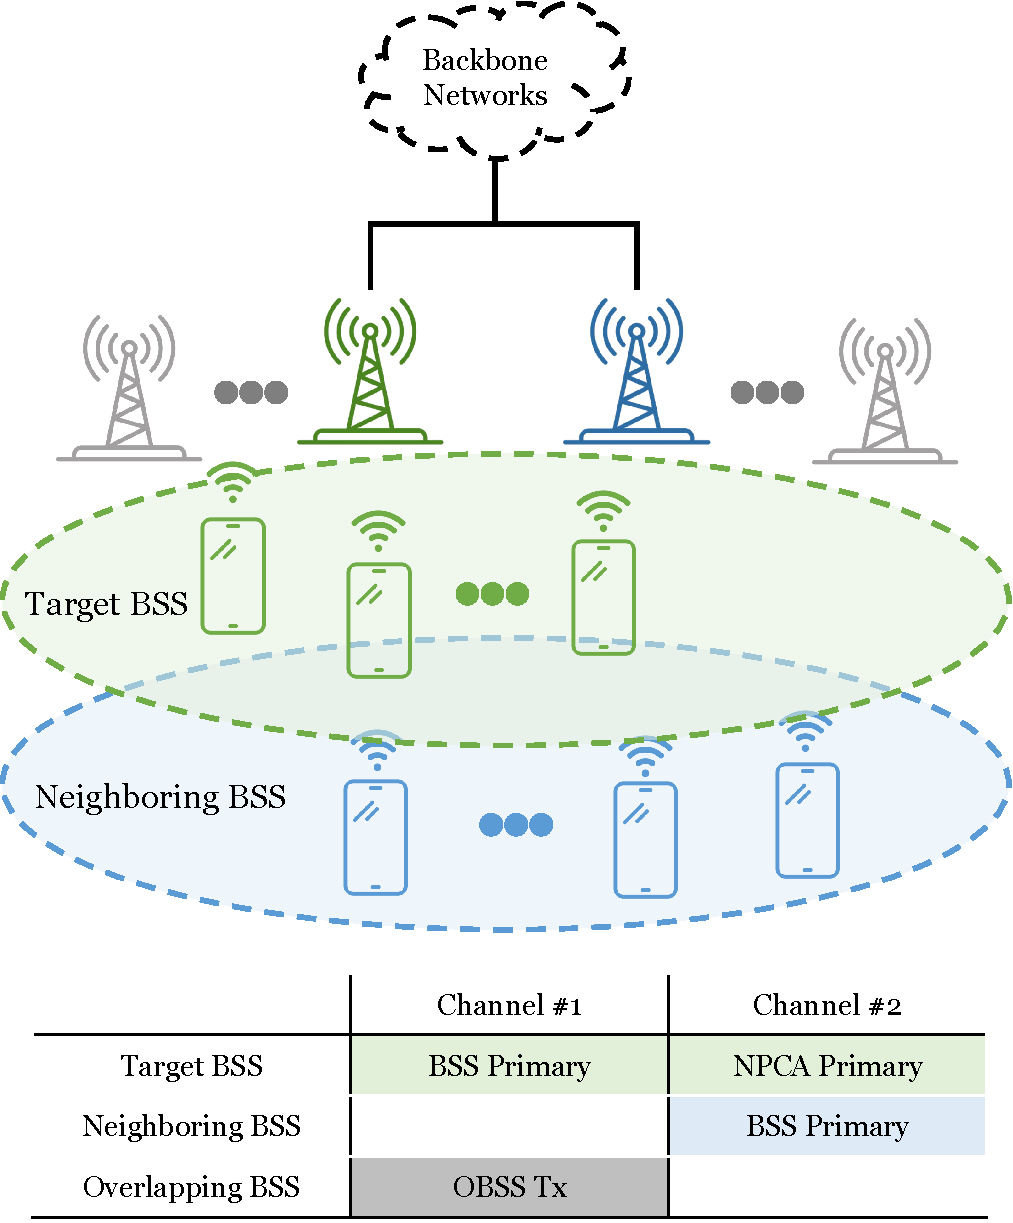
\includegraphics[width=0.45\textwidth]{figure/topology_and_channel.pdf}
    \caption{Two-BSS topology and channel assignment.}
    \label{fig:topology_and_channel}
\end{figure}

Fig.~\ref{fig:topology_and_channel} depicts the two-BSS topology and channel assignment assumed throughout this work. The target BSS, whose NPCA operation is our focus, comprises an access point (AP) and a set $\mathcal{V}=\{1,2,\dots,\Nvis\}$ of associated non-AP STAs and they can be considered as \emph{visitors} to the neighboring BSS. The visitors normally contend on their BSS primary channel, Channel~\#1 in Fig.~\ref{fig:topology_and_channel}, which is the main channel used by the target BSS for its own transmissions.

Channel~\#1 is also used by an OBSS operating on the same channel, whose transmissions intermittently render it busy. In standards prior to IEEE 802.11bn, a STA could not initiate a transmission whenever its designated primary channel was busy, even if the secondary channel was idle.
In IEEE 802.11bn, however, the AP can designate a separate channel as the NPCA primary channel, used by the visitors during NPCA operation, named as Channel~\#2 in Fig.~\ref{fig:topology_and_channel}. We use the qualifier ``BSS'' to distinguish the original primary channel from the NPCA primary channel, consistent with P802.11bn Draft terminology~\cite{ieee80211bn}.

The NPCA primary channel is not unused spectrum reserved for the target BSS. Channel~\#2 is itself the BSS primary channel of the neighboring BSS, comprising its own AP and a set $\mathcal{N}=\{1,2,\dots,\Nnat\}$ of \emph{native} STAs that contend on it with standard DCF at all times. The visitors, by contrast, use Channel~\#2 only opportunistically, during NPCA visits. Two classes of contenders therefore coexist on the NPCA primary channel: the native STAs, which contend there persistently, and the visitors, whose access is confined to the bounded NPCA window.

As depicted in Fig.~\ref{fig:topology_and_channel}, we assume the coverages of the two BSSs coincide, so that all visitors and native STAs are mutually within carrier-sensing range and form a single collision domain on the NPCA primary channel: every visitor senses, defers to, and competes with every native STA. This is the configuration in which the visitors' impact on native airtime is greatest, so the coexistence results reported here upper-bound that cost. In general the two coverages may overlap only partially, in which case a visitor outside the neighboring BSS coverage would reuse the NPCA primary channel without contending with the natives at all; this spatial-reuse regime only lowers the coexistence cost and is left to future work. 

\begin{figure}
    \centering
    
\includegraphics[width=0.48\textwidth]{figure/channel_access.pdf}
    \caption{The medium access process comparison with and without NPCA.}
    \label{fig:channel_access}
\end{figure}

\subsection{NPCA Operation and Effective Window}
\label{subsec:npca_access}

Fig.~\ref{fig:channel_access} contrasts the medium-access processes with and without NPCA operation. Under conventional access (top), prior to IEEE 802.11bn, a STA contends only on the BSS primary channel.\footnote{We use the term BSS primary channel to distinguish the original primary channel from the NPCA primary channel introduced in IEEE 802.11bn. Prior to 802.11bn, when NPCA was not yet defined, this channel was referred to simply as the primary channel.} It decrements its backoff counter while the channel is idle and transmits when the counter reaches zero. If the secondary channel is also sensed idle at this instant, the STA may bond it with the BSS primary channel and transmit a wideband PPDU spanning the combined bandwidth (e.g., $40$, $80$, $160$, or $320$~MHz). When an OBSS transmission seizes the BSS primary channel, however, the STA must defer and freeze its backoff for the entire OBSS busy period, even though the secondary channel is idle.

Under NPCA access (bottom), a STA no longer wastes the OBSS busy period. When it detects an OBSS transmission on the BSS primary channel, it decodes the preamble of that transmission and learns its duration in advance,\footnote{NPCA relies on preamble detection rather than energy detection. A STA must decode the inter-BSS PPDU preamble at PHY-RXSTART to both classify the transmission and derive its remaining duration, from which the NPCA window is determined. Energy detection alone, which yields no length or BSS information, is insufficient to trigger an NPCA transition.} rather than freezing its backoff for the whole period, it switches to the idle NPCA primary channel and contends and transmits there. On each such switch the STA saves its backoff state on the BSS primary channel and initializes a fresh contention window for the NPCA primary channel, so every NPCA visit begins at the minimum backoff stage regardless of prior history. The STA already knows when the OBSS transmission will finish, so it sets a timer to that instant and switches back to the BSS primary channel when the timer expires, restoring the saved state without having to re-sense the channel. In this way the secondary spectrum that the a conventional STA leaves idle is put to use, and a STA can complete one or more transmissions that it would otherwise have had to postpone.

Two constraints shape this access. First, a radio transition delay $\delta_\mathrm{sw}$ is incurred on each switch: the STA becomes ready on the NPCA primary channel only after the switching delay, and the NPCA timer is set to expire one switch-back delay before the OBSS transmission ends so that the STA is back on the BSS primary channel in time~\cite{ieee80211bn}. Second, the opportunity lasts only until the known end of the OBSS transmission, whose remaining duration $D_\mathrm{rem}$ is read from the preamble. Contention and transmission must therefore fit within a bounded window of
\begin{equation}
    W_\mathrm{eff} \;=\; \left\lfloor
    \frac{D_\mathrm{rem}-2\,\delta_\mathrm{sw}}{\sigma} \right\rfloor
    \quad\text{slots},
    \label{eq:weff}
\end{equation}
where $\sigma$ is the slot time, typically $9$~$\mu$s in IEEE 802.11-compliant systems. Hence, a single NPCA transition admits NPCA transmissions during $W_\mathrm{eff}$ slots at most, which we index by $t \in \{1, 2, \dots, W_\mathrm{eff}\}$. 

This deadline is the crux of NPCA. Every backoff decision competes against it. A STA that collides doubles its contention window as usual, and once the resulting backoff exceeds the slots left in $W_\mathrm{eff}$, it can no longer transmit before the window closes so it wastes the rest of the opportunity despite having data to send.

Because the contention window is reset at every NPCA visit, this penalty recurs each time rather than amortizing across visits. This mismatch between open-ended backoff and the finite window is the inefficiency that PACE targets.

\subsection{Slotted Contention Model}
\label{subsec:npca_window}

We model time on the NPCA primary channel as a sequence of slots of duration $\sigma$. Each visitor maintains a per-slot transmission probability $\tau_i(t)$ at each time slot $t$ and, when eligible, transmits in slot $t$ with that probability, in the manner of slotted ALOHA; we abbreviate it as $\tau_i$ where the slot index is immaterial. This per-slot access probability is the variable that the scheme of Section~\ref{sec:pace_algorithm} controls. The standard baseline instead runs its backoff countdown unchanged, and enters the model only through the slot outcomes defined below.

This probabilistic access departs from the current draft, which reuses
the enhanced distributed channel access (EDCA) backoff procedure on the NPCA primary channel~\cite{ieee80211bn}. PACE keeps the NPCA architecture intact, including the switching triggers, the NPCA timer, and the contention-state save and restore, and replaces only the contention rule applied within the bounded visit. 
% We therefore position PACE as a candidate refinement of the amendment's contention rule, whose benefit over the draft-compliant procedure is quantified in Section~\ref{sec:performance_evaluation}.

Following the slot indexing $t\in\{1,\dots,W_\mathrm{eff}\}$ of Section~\ref{subsec:npca_access}, we denote by $W_\mathrm{rem}(t)=W_\mathrm{eff}-t+1$ the number of slots remaining at slot $t$, including the current one, so that $W_\mathrm{rem}$ counts down toward the deadline as contention proceeds. All STAs are assumed to be saturated, so each STA $i$ always holds a pending head-of-line PPDU, whose transmission occupies $L_i$ slots, and a STA that completes a transmission draws its next frame and continues contending. $L_i$ therefore changes only at STA $i$'s own delivery instants and is constant in between; we suppress this time dependence in the notation and let $L_i$ always denote the current head-of-line frame. Because a transmission must complete before the window closes, STA $i$ is viable at slot $t$ only if its frame still fits, i.e.\ $L_i \le W_\mathrm{rem}(t)$; otherwise it can no longer succeed within the visit. We write the viable population at slot $t$ as
\begin{equation}
    \mathcal{V}(t) \;=\; \bigl\{\, i\in\mathcal{V} :
    L_i \le W_\mathrm{rem}(t) \,\bigr\},
    \label{eq:viable}
\end{equation}
which is non-increasing in $t$ as both the window depletes and frames become infeasible.

The viable population defines a natural operating point for contention. In a slot with $|\mathcal{V}(t)|$ viable STAs each attempting independently with a common probability, a success, meaning exactly one transmitter, is most likely when that probability is
\begin{equation}
    \tau^*(t) \;=\; \frac{1}{|\mathcal{V}(t)|},
    \label{eq:tau_opt}
\end{equation}
the classical slotted-ALOHA optimum applied to the viable set. This is the attempt-fair operating point rather than an airtime optimum, and it is the target the scheme of Section~\ref{sec:pace_algorithm} tracks in service of the efficiency and fairness objective of Section~\ref{subsec:factor_scaling}. Because $\mathcal{V}(t)$ is non-increasing, the target rises toward the deadline, and tracking it without knowing $|\mathcal{V}(t)|$ is what Section~\ref{sec:pace_algorithm} constructs.

At each slot $t$, a viable STA $i$ attempts transmission with probability $\tau_i(t)$. Following the half-duplex assumption, a transmitting STA cannot sense the channel in the same slot. Let $\mathcal{D}(t)$ denote the set of STAs whose transmissions on the NPCA primary channel are detected by a given STA in slot $t$. This set is defined at the channel level. It counts every STA transmitting on that channel in the slot, not only the switching visitors but also any other STA that uses the same channel as its own primary. The slot outcome is idle when $|\mathcal{D}(t)|=0$, a success when $|\mathcal{D}(t)|=1$, and a collision when $|\mathcal{D}(t)|\ge 2$. These three observable events are the only feedback available to a STA, and they drive the adaptive contention control developed in Section~\ref{sec:pace_algorithm}.

The remaining window advances by the time each outcome occupies the medium. An idle slot consumes one slot, while a successful slot consumes $L_\mathrm{solo}$ slots and a collision consumes $L_\mathrm{col}$ slots. The two occupancies depend on the access mode.

\subsubsection{Basic Access}
A successful slot is occupied by the sole sender's frame,
\begin{equation}
    L_\mathrm{solo} \;=\; L_i \quad \text{if } \mathcal{D}(t)=\{i\},
    \label{eq:lsolo_basic}
\end{equation}
while a collision keeps the medium busy until the longest colliding frame has ended,
\begin{equation}
    L_\mathrm{col} \;=\; \max_{i\in\mathcal{D}(t)} L_i,
    \label{eq:lmax}
\end{equation}
as in standard IEEE 802.11 without collision detection. Since each STA contends for one head-of-line PPDU at a time, $L_i$ is fixed until that frame is delivered; the slot dependence of both occupancies enters through the identity of the transmitters $\mathcal{D}(t)$ and their current frames.

\subsubsection{RTS/CTS-Protected Access}
Under RTS/CTS-protected access the busy-slot accounting changes. A successful exchange is preceded by the handshake and therefore occupies
\begin{equation}
    L_\mathrm{solo} \;=\; L_i + L_\mathrm{hs} \quad \text{if } \mathcal{D}(t)=\{i\},
    \label{eq:lsolo_rts}
\end{equation}
slots, where
\begin{equation}
    L_\mathrm{hs} \;=\; \left\lceil
    \frac{T_\mathrm{RTS} + T_\mathrm{CTS} + 2\,T_\mathrm{SIFS}}{\sigma}
    \right\rceil
    \label{eq:oh_rts}
\end{equation}
is the handshake overhead, with $T_\mathrm{RTS}$, $T_\mathrm{CTS}$, and $T_\mathrm{SIFS}$ being the RTS, CTS, and short interframe space (SIFS) durations defined in IEEE 802.11. A collision, by contrast, involves only RTS frames. The data frames are never sent, and the channel recovers after the extended interframe space, so a collision occupies
\begin{equation}
    L_\mathrm{col} \;=\; \left\lceil
    \frac{T_\mathrm{RTS} + T_\mathrm{EIFS}}{\sigma} \right\rceil
    \label{eq:coll_rts}
\end{equation}
slots, where $T_\mathrm{EIFS}=T_\mathrm{SIFS}+T_\mathrm{ACK}+T_\mathrm{DIFS}$ is the extended interframe space with $T_\mathrm{ACK}$ and $T_\mathrm{DIFS}$ being the acknowledgment (ACK) and distributed interframe space (DIFS) durations defined in IEEE 802.11. Unlike its basic-access counterpart of~\eqref{eq:lmax}, this occupancy is a constant, independent of the colliding frame lengths and of the slot index. Under protection the viability test of~\eqref{eq:viable} must also leave room for the handshake, i.e.\ $L_i$ is replaced by $L_i+L_\mathrm{hs}$. Basic access is recovered as the special case $L_\mathrm{hs}=0$ with $L_\mathrm{col}$ given by~\eqref{eq:lmax}. Both access modes are evaluated in Section~\ref{subsec:eval_whypace}.

\section{PACE Algorithm}
\label{sec:pace_algorithm}

\begin{figure}
    \centering
    \begin{subfigure}{\linewidth}
        \centering
        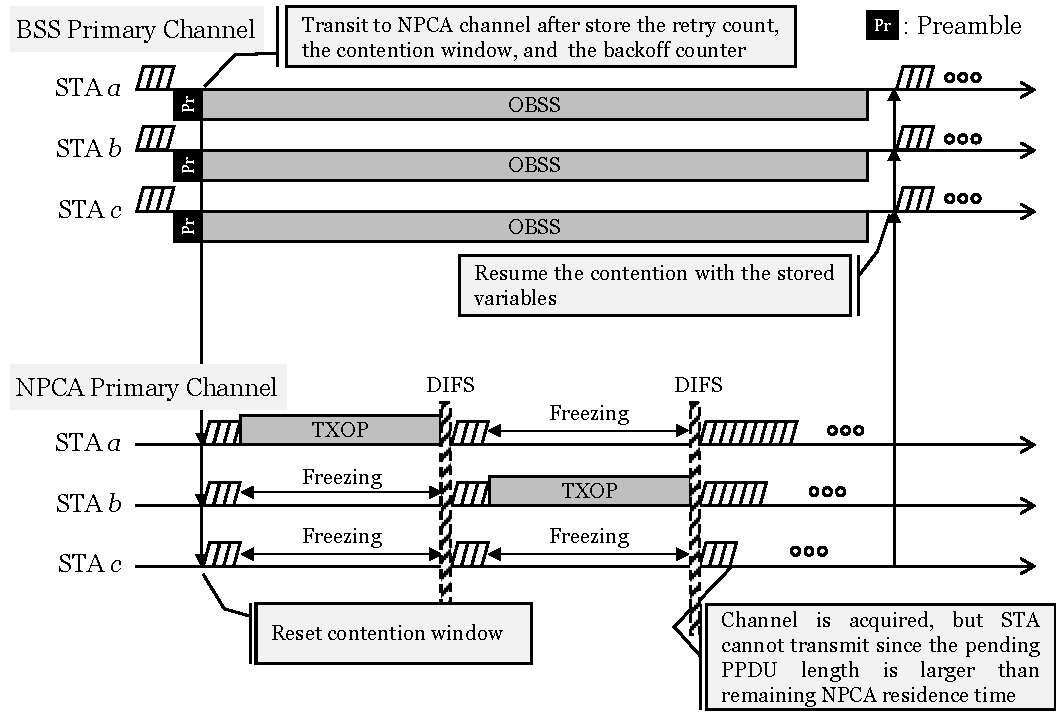
\includegraphics[width=\linewidth]{figure/transition_npca.pdf}
        \caption{NPCA baseline (BEB).}
        \label{fig:transition_npca}
    \end{subfigure}
    \\[1.5ex]
    \begin{subfigure}{\linewidth}
        \centering
        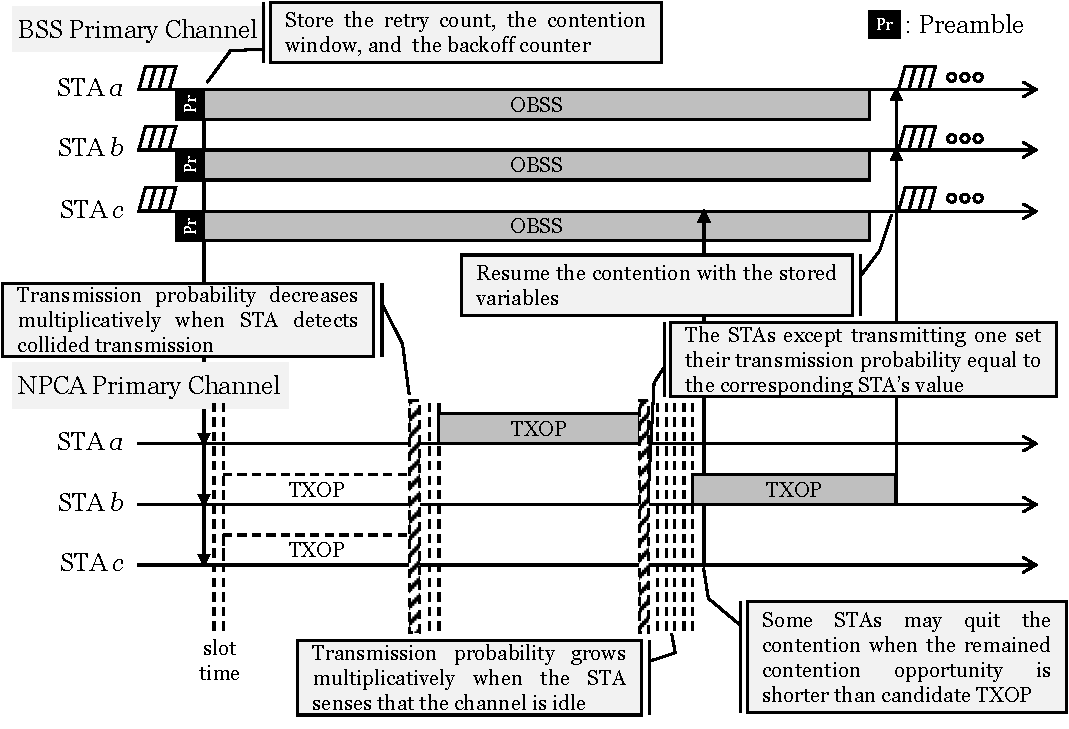
\includegraphics[width=\linewidth]{figure/transition_pace.pdf}
        \caption{Proposed PACE (probabilistic adaptive contention).}
        \label{fig:transition_pace}
    \end{subfigure}
    \caption{Medium access on the NPCA primary channel: a STA that detects
    an OBSS transmission on the BSS primary channel migrates and contends within
    the bounded NPCA window. (a) the standard NPCA baseline with binary
    exponential backoff, and (b) the proposed PACE with probabilistic adaptive
    contention and PPDU-aware self-exclusion.}
    \label{fig:contention}
\end{figure}

Fig.~\ref{fig:contention} illustrates contention on the NPCA primary channel under the slotted model of Section~\ref{subsec:npca_window} and contrasts the two schemes studied in this paper. In both, a STA that detects an OBSS transmission on the BSS primary channel stores its DCF state, migrates to the NPCA primary channel, and contends there until the NPCA timer expires, whereupon it restores the saved state and resumes on the BSS primary channel. Under the NPCA baseline of Fig.~\ref{fig:transition_npca}, STAs contend with BEB. A STA that collides doubles its contention window, so its counter can outlast the remaining window, and because the countdown is frozen during every busy period, the surviving counters tend to expire together and collide again.

Meanwhile, under the proposed PACE scheme of Fig.~\ref{fig:transition_pace}, each STA instead adapts its per-slot probability $\tau_i$ from the idle, success, and collision feedback. The access probability is raised multiplicatively on idle slots, lowered on collisions, and replaced by the successful sender's value on solo receptions. In addition, a STA proactively withdraws from contention once its frame can no longer fit within $W_\mathrm{rem}(t)$.

\begin{algorithm}[t]
\caption{PACE at STA $i$ during one NPCA visit}
\label{alg:pace}
\begin{algorithmic}[1]
\REQUIRE head-of-line PPDU length $L_i$ (slots), window $W_\mathrm{eff}$, factors $c_\mathrm{coll},\,c_\mathrm{idle}>1$, handshake overhead $L_\mathrm{hs}$ of Eq.~\eqref{eq:oh_rts} ($L_\mathrm{hs}=0$ under basic access)
\PHASE {/* Phase (a): Probability Initialization */}
\STATE $\tau_i \leftarrow 1/W_\mathrm{eff}$;\quad $W_\mathrm{rem} \leftarrow W_\mathrm{eff}$
\WHILE{$W_\mathrm{rem} > 0$}
    \PHASE {/* Phase (b): PPDU-aware Self-Exclusion */}
    \IF{$L_i + L_\mathrm{hs} > W_\mathrm{rem}$}
        \STATE $\tau_i \leftarrow 0$
    \ENDIF
    \PHASE {/* Phase (c): Probabilistic Channel Access */}
    \STATE draw $u \sim \mathrm{Uniform}(0,1)$
    \IF{$u < \tau_i$}
        \STATE transmit the PPDU, advertising $\tau_i$ (preceded by the RTS/CTS handshake under protected access)
        \IF{solo success}
            \STATE $W_\mathrm{rem} \leftarrow W_\mathrm{rem} - L_\mathrm{solo}$;\quad $L_i \leftarrow$ next pending PPDU
        \ELSE
            \STATE $W_\mathrm{rem} \leftarrow W_\mathrm{rem} - L_\mathrm{col}$ \COMMENT{collided: Eq.~\eqref{eq:coll_rts} under protection, Eq.~\eqref{eq:lmax} under basic access}
        \ENDIF
    \ELSE
        \PHASE {/* Phase (d): Feedback-based Adaptation */}
        \STATE observe the slot outcome $|\mathcal{D}(t)|$
        \IF{$|\mathcal{D}(t)| = 0$}
            \STATE $\tau_i \leftarrow \min(\tau_i \cdot c_\mathrm{idle},\;1)$;\quad $W_\mathrm{rem} \leftarrow W_\mathrm{rem} - 1$
        \ELSIF{$|\mathcal{D}(t)| = 1$ where $\mathcal{D}(t) = \{j\}$}
            \STATE $\tau_i \leftarrow \tau_j$ \COMMENT{the solo sender's advertised probability};\quad $W_\mathrm{rem} \leftarrow W_\mathrm{rem} - L_\mathrm{solo}$
        \ELSE
            \STATE $\tau_i \leftarrow \tau_i / c_\mathrm{coll}$;\quad $W_\mathrm{rem} \leftarrow W_\mathrm{rem} - L_\mathrm{col}$
        \ENDIF
    \ENDIF
\ENDWHILE
\end{algorithmic}
\end{algorithm}

Algorithm~\ref{alg:pace} summarizes PACE as executed independently by each STA on the NPCA primary channel during a single NPCA visit. Every STA runs the same rule using only locally observable feedback, those are, the per-slot outcome and its own remaining window without central coordination or knowledge of the contending population.

% Algorithm~\ref{alg:pace} is expressed in the per-slot transmission-probability
% model of Section~\ref{subsec:npca_window}. A viable STA transmits in a slot
% with probability $\tau_i$. This is a probabilistic, slotted-ALOHA-style access
% policy.

We adopt the probabilistic approach for two reasons. First, the
per-slot probability $\tau$ is the common abstraction under which DCF, PND, and
AND are all analyzed~\cite{bianchi2000performance,song2014pnd,vasudevan2013efficient},
so it places PACE on the same analytical footing as these schemes.
Second, and more fundamentally, the finite NPCA window is precisely
where a deterministic countdown breaks down. A single backoff draw cannot
re-adapt within the handful of slots a visit lasts, whereas a per-slot
probability can be re-steered every slot by the feedback law, which will be described in Subsec.~\ref{subsec:adaptive_control}. The
ALOHA-style attempt is therefore not incidental but the mechanism that makes
within-window adaptation possible.

Algorithm~\ref{alg:pace} runs four phases per visit. (a) a one-time probability
initialization, followed by a per-slot loop of (b) self-exclusion, (c) channel
access, and (d) feedback-based adaptation. The remainder of this section develops
each phase in turn.

\subsection{Phase (a): Probability Initialization}
\label{subsec:init}

A visitor that has just switched to the NPCA primary channel does not know how
many other STAs are contending there. The population-matched choice
$\tau_0=1/(\Nvis{+}\Nnat)$, which is the value the target $\tau^*$ of Eq.~\eqref{eq:tau_opt} takes at the start of a visit in which every contender fits, is therefore unavailable in practice since the contender count is not observable.

Visitor STAs might, through association state or management traffic, form some
estimate of how many STAs belong to its own BSS. The harder obstacle is that
the population it actually contends with also includes the native STAs of the
neighboring BSS that owns the NPCA primary channel. That is, a visitor competes against these as well, yet has no direct way to learn how many are active. The count that would
parameterize $1/(\Nvis{+}\Nnat)$ is thus doubly hidden, which motivates a surrogate that
avoids counting STAs altogether.

We propose a method where the window length itself determines the scale. A visit spans $W_\mathrm{eff}$ slots, and a STA contends in at most one of them per slot so $W_\mathrm{eff}$ upper-bounds the number of attempt opportunities any STA sees in a visit. A STA attempting with probability $\tau$ therefore expects at most $W_\mathrm{eff}\,\tau$ attempts before the deadline. Fixing this budget to a single probe per STA, $W_\mathrm{eff}\,\tau_0 = 1$ sets the most conservative self-consistent  exploration rate. Low enough to avoid an early collision storm, yet high enough for each STA to test the medium about once before the window drains. This yields
\begin{equation}
    \tau_0 = \frac{1}{W_\mathrm{eff}},
    \label{eq:init}
\end{equation}
with which each visitor starts the visit, $\tau_i(1)=\tau_0$. It depends only on the effective window $W_\mathrm{eff}$, which is a quantity that each STA can compute locally from the OBSS PPDU duration and no knowledge of the contender count is required.

In general frame length to be transmitted on NPCA primary channel is longer than a single slot, so $\tau_0 $ is bound to be smaller than the optimal value. This choice is deliberately biased toward under-attempting for two reasons. First, it is self-correcting in the safe direction. An over-conservative $\tau_i$ is raised toward the operating point within a few slots by the idle-driven multiplicative increase in Phase~(d), whereas an over-aggressive start triggers collisions whose wasted slots cannot be reclaimed inside a finite window. The MIMD recovery is thus asymmetric, and starting low pays only a bounded ramp-up cost. Second, $1/W_\mathrm{eff}$ tracks the regime where initialization matters most. When the window is tight, i.e., $W_\mathrm{eff}\!\approx\!\Nvis{+}\Nnat$, it already approximates the optimum $1/(\Nvis{+}\Nnat)$, and when the window is loose such as $W_\mathrm{eff}\!\gg\!\Nvis{+}\Nnat$, the mild initial timidity is erased by the idle increase long before the window drains. 
% Section~\ref{sec:performance_evaluation} shows that this locally computable initialization stays within a few percent of the count-aware optimum across the entire window-tightness range, while aggressive or wide-spread initializations collapse---confirming that PACE inherits the initialization-robustness of neighbor discovery only when the initial scale is kept at or below $1/W_\mathrm{eff}$.

\subsection{Phase (b): PPDU-aware Self-Exclusion}
\label{subsec:self_exclusion}

At the start of every slot a STA applies a frame-fit test, comparing the airtime its own frame needs to the remaining window $W_\mathrm{rem}(t)$. Following the viability condition of Eq.~\eqref{eq:viable}, that airtime is $L_i$ under basic access and $L_i+L_\mathrm{hs}$ under RTS/CTS protection, since the handshake of Eq.~\eqref{eq:oh_rts} must also fit before the deadline. If the frame can no longer finish, the STA sets $\tau_i(t)=0$ and stays out of the slot. The test is repeated at every subsequent slot, and because $W_\mathrm{rem}(t)$ only shrinks the STA remains silent for the rest of the visit unless it later holds a shorter frame. The test involves only the STA's own frame and the slot index and thus, like initialization, requires no knowledge of the contending population.

Conventional NPCA has no such rule, yet the deadline binds it all the same, since a STA shall switch back to the BSS primary channel when the NPCA timer expires~\cite{ieee80211bn}. A frame that does not fit the remaining window is therefore cut off at expiry even if it wins the channel; self-exclusion makes this inevitability explicit and returns those slots to the STAs that can still finish.

Self-exclusion keeps the optimal target $\tau^*(t)$ of Eq.~\eqref{eq:tau_opt}, which PACE aims to track, meaningful in a heterogeneous and finite window. A STA whose frame no longer fits is removed from the viable set $\mathcal{V}(t)$ of Eq.~\eqref{eq:viable}, so it neither wastes time on attempts destined to fail nor inflates the contention seen by the STAs that can still succeed. This plays the same role as the collision detection departure of a previously proposed neighbor discovery algorithm~\cite{song2014pnd}, in which a STA leaves the contention once its advertisement succeeds. Here a STA also leaves once its frame provably cannot complete, tightening $\mathcal{V}(t)$ toward the set of STAs that genuinely compete for the remaining slots.

\subsection{Phase (c): Probabilistic Channel Access}
\label{subsec:channel_access}

A STA that is still viable transmits in slot $t$ with probability $\tau_i(t)$ and otherwise listens. Because the radio is half-duplex, a transmitting STA cannot sense the slot it occupies. It learns from the acknowledgement whether its own frame got through, which tells it how far the window has advanced and whether to dequeue the next frame, but it observes none of the three slot outcomes that drive the adaptation, so it leaves $\tau_i$ untouched on its own transmissions. Each transmitted PPDU advertises the sender's current $\tau_i(t)$ in its header\footnote{A few quantization bits for $\tau_i$ fit in the Control Information field of a newly defined A-Control subfield, identified by a new Control ID, of the HT Control field that rides unencrypted in the MAC header of a QoS Data frame. Defining such a subfield would require an IEEE~802.11 amendment, but follows the existing A-Control extension framework. One placement serves both access modes, since RTS and CTS carry no HT Control field and a solo success propagates $\tau_i$ only once the QoS Data MPDU is decoded.}, which the listeners use in Phase~(d). This value describes only the sender's own state and rides in a frame it transmits anyway, in the manner of the per-frame information IEEE~802.11 headers already carry, so no control frame is added and no STA ever learns how many others are contending.

A slot is a success when exactly one viable STA transmits and its frame fits the remaining window. Being saturated, the winner then draws its next pending frame and re-enters the contention with its current $\tau_i$, which the solo advertisement has just propagated to the listeners; the viable set $\mathcal{V}(t)$ therefore shrinks only through self-exclusion as the deadline nears. Slots with no transmission are idle, and slots with two or more transmissions are collisions; both outcomes are observed by every non-transmitting STA and feed the adaptation of Phase~(d).

\subsection{Phase (d): Feedback-based Adaptation}
\label{subsec:adaptive_control}

Every STA that listened in slot $t$ updates its probability from the slot outcome $|\mathcal{D}(t)|$ using the MIMD rule inherited from neighbor discovery as
\begin{equation}
\tau_i(t') =
\begin{cases}
\min\bigl(c_\mathrm{idle}\,\tau_i(t),\,1\bigr) & |\mathcal{D}(t)|=0\;(\text{idle}),\\[2pt]
\tau_j(t)              & \mathcal{D}(t)=\{j\}\;(\text{success}),\\[2pt]
\tau_i(t) / c_\mathrm{coll}          & |\mathcal{D}(t)|\ge 2\;(\text{collision}),
\end{cases}
\label{eq:mimd}
\end{equation}
with $c_\mathrm{idle},c_\mathrm{coll}>1$, where $t'$ denotes the next contention slot after the outcome of slot $t$, i.e., $t'=t+1$ after an idle slot and $t'=t+L_\mathrm{solo}$ or $t'=t+L_\mathrm{col}$ after a busy one, and $\tau_i$ is unchanged while the medium is occupied. 

An idle slot signals that the
population has been overestimated and the attempt rate is raised by the factor of $c_\mathrm{idle}$. On the other hand, a collision signals the opposite, hence, once STAs detect a collision, the attempt rate is divided by $c_\mathrm{coll}$ to reduce the contention. On a solo success, every listener copies the advertised $\tau_j$, so a single successful slot propagates the winning operating point to the whole contending set at once, giving PACE the fast intra-visit consensus.

None of the three updates counts the viable STAs. Instead, the idle and collision statistics move each $\tau_i$ toward the operating point implicitly, and solo-copy pulls the population onto a common value, so the ensemble approximately tracks the time-varying optimum $\tau^*(t)$ of Eq.~\eqref{eq:tau_opt} without estimating the number of contending STAs $|\mathcal{V}(t)|$. 

The direction of this adaptation is what separates PACE from BEB. Because the viable set only shrinks over a visit, the optimal target $\tau^*(t)=1/|\mathcal{V}(t)|$ of~\eqref{eq:tau_opt} rises as the deadline approaches. On the other hand, the BEB moves the opposite way, that is, a collision doubles the contention window and halves the attempt rate, so the access probability falls exactly when it should climb.

Finally, the rule of Eq.~\eqref{eq:mimd} needs no modification to operate alongside the native STAs of Section~\ref{subsec:network_model}. Because the slot outcome $\mathcal{D}(t)$ is measured at the channel level, native activity enters a visitor's feedback directly. A slot in which two or more frames overlap is a collision whether the extra transmitter is a visitor or a native, so a native transmission that clashes with a visitor lowers that visitor's $\tau_i$, and a slot with no transmission at all, native or visitor, is idle and raises it. The solo case is the one exception. The copy $\tau_i(t') = \tau_j(t)$ requires the successful frame to advertise a probability, which only a PACE visitor does; when a native transmits alone, its frame carries no such value, so a listening visitor keeps $\tau_i$ unchanged and simply observes the busy slot while the window continues to shrink.

% The mismatch is twofold. First, the adaptation is backwards---BEB retreats on congestion while the window's diminishing population
% calls for a more aggressive attempt rate---so late slots are left idle. Second,
% the doubled backoff can exceed the remaining window $W_\mathrm{rem}(t)$,
% silencing the STA for the rest of the visit and wasting those slots
% outright; unlike PACE's self-exclusion, which silences only STAs that
% provably cannot finish, this dead time falls on STAs that could still have
% succeeded. PACE's idle-increase and solo-copy instead move $\tau_i$ along the
% rising $\tau^*(t)$ trajectory, matching the sign of the optimal policy rather
% than fighting it.

\subsection{Window Scaling of the Adaptation Factors}
\label{subsec:factor_scaling}

The rule of Eq.~\eqref{eq:mimd} leaves the factors $c_\mathrm{idle}$ and $c_\mathrm{coll}$ open, and the finite window turns their choice into a trade-off between two losses that both accumulate before the deadline. A small factor adapts slowly and spends the visit ramping toward the operating point, whereas a large one reaches it quickly but keeps overshooting around it. This subsection quantifies the balance by treating Phase~(d) as a finite-horizon stochastic approximation. We set the two factors equal, which keeps every $\tau_i$ on a common multiplicative grid so that the solo-copy of Eq.~\eqref{eq:mimd} exchanges values the listeners can themselves reach, and the pair then reduces to a single log-domain step size
\begin{equation}
    \epsilon \;=\; \ln c_\mathrm{idle} \;=\; \ln c_\mathrm{coll}.
    \label{eq:logstep}
\end{equation}

Let $X_k=\ln\tau_i$ at the $k$-th update opportunity of a visit. Under Eq.~\eqref{eq:mimd} the state performs a random walk $X_{k+1}=X_k+\epsilon H_k$, where $H_k$ equals $+1$ on an idle outcome, $-1$ on a collision, and $0$ otherwise. The mean drift $h(x)=p_\mathrm{I}(x)-p_\mathrm{C}(x)$, the gap between the idle and collision probabilities seen from state $x$, vanishes at the operating point $x^*$ that the feedback seeks. Near a stable $x^*$ the error $Y_k=X_k-x^*$ follows the linearized recursion
\begin{equation}
    Y_{k+1} \;\approx\; (1-\kappa\epsilon)\,Y_k + \epsilon\,\xi_{k+1},
    \label{eq:linrec}
\end{equation}
with restoring rate $\kappa=-h'(x^*)>0$ and zero-mean outcome noise $\xi$ of variance $\nu^2=p_\mathrm{I}(x^*)+p_\mathrm{C}(x^*)$.

A visit is scored by what it accumulates rather than by where it ends. We make the objective explicit as
\begin{equation}
    J \;=\; \ln T \;-\; \alpha\,\bigl(\ln\rho\bigr)^{2},
    \label{eq:objective}
\end{equation}
where $T$ is the fraction of the window carrying useful airtime, $\rho$ is the visitors' share of that airtime divided by their population share $\Nvis/(\Nvis{+}\Nnat)$, and $\alpha\ge0$ weights proportionality against efficiency. The quadratic log penalty vanishes exactly at the proportional share $\rho=1$ and charges over- and under-service symmetrically, so $J$ scores the design goal of Section~\ref{subsec:self_exclusion}, an efficient window that neither starves the visitors nor lets them displace the natives. Both ingredients accumulate over the whole window and are the measures that Section~\ref{sec:performance_evaluation} reports. Treating $J$ as a function of the operating point and assuming it is locally quadratic around $x^*$ with curvature $q>0$, summing the second moment of Eq.~\eqref{eq:linrec} over the $K$ update opportunities of a visit gives the loss
\begin{equation}
    R_K(\epsilon) \;\approx\; \frac{q}{4\kappa}
    \left( \frac{Y_0^2}{\epsilon} + K \nu^2 \epsilon \right),
    \label{eq:regret}
\end{equation}
where $Y_0$ is the initial offset. The first term is the transient cost of a slow ramp and decays as $1/\epsilon$, while the second is the fluctuation that a large step sustains around the operating point and grows as $K\epsilon$. The two scale oppositely in $\epsilon$, and balancing them yields
\begin{equation}
    \epsilon^* \;=\; \frac{|Y_0|}{\nu\sqrt{K}}.
    \label{eq:eps_opt}
\end{equation}

The number of update opportunities is in turn set by the window. Every outcome occupies the medium for one idle slot, $L_\mathrm{solo}$ slots, or $L_\mathrm{col}$ slots, so $K\approx W_\mathrm{eff}/\bar{L}$, where $\bar{L}$ is the mean outcome occupancy of the access mode in use. Substituting into Eq.~\eqref{eq:eps_opt},
\begin{equation}
    \epsilon^* \;=\; \frac{C}{\sqrt{W_\mathrm{eff}}},
    \qquad
    C \;=\; \frac{|Y_0|\sqrt{\bar{L}}}{\nu},
    \label{eq:eps_window}
\end{equation}
which prescribes $c_\mathrm{idle}^*=c_\mathrm{coll}^*=\exp\bigl(C/\sqrt{W_\mathrm{eff}}\,\bigr)$. The constant also separates the two access modes. Since basic access and RTS/CTS protection differ through $L_\mathrm{solo}$ and $L_\mathrm{col}$, their constants relate as $C_\mathrm{RTS}/C_\mathrm{basic}\approx\sqrt{\bar{L}_\mathrm{RTS}/\bar{L}_\mathrm{basic}}$, so the mode whose outcomes hold the channel longer, and hence grants fewer updates per window, calls for a proportionally larger step. The argument is summarized as follows.

\begin{proposition}
Consider the finite-horizon adaptation $X_{k+1}=X_k+\epsilon H_k$ with a locally stable equilibrium $x^*$, a locally quadratic utility, and bounded outcome noise of variance $\nu^2$. If a visit contains $K$ effective update opportunities and both the transient and the fluctuation loss of Eq.~\eqref{eq:regret} are accumulated, the loss-minimizing constant step satisfies
\begin{equation*}
    \epsilon^*_K \;=\; \frac{|X_0-x^*|}{\nu\sqrt{K}} + o\bigl(K^{-1/2}\bigr),
\end{equation*}
hence $\epsilon^*_K=\Theta(K^{-1/2})$. If moreover $K=W_\mathrm{eff}/\bar{L}+o(W_\mathrm{eff})$, then $\epsilon^*=C/\sqrt{W_\mathrm{eff}}+o\bigl(W_\mathrm{eff}^{-1/2}\bigr)$ with $C$ as in Eq.~\eqref{eq:eps_window}.
\end{proposition}

Two remarks bound the claim. First, Phase~(a) sets $X_0=-\ln W_\mathrm{eff}$, so the offset $|Y_0|=|\ln(W_\mathrm{eff}\,\tau^*)|$ retains a slow logarithmic dependence on the window, and $C$ behaves as a constant only over ranges of $W_\mathrm{eff}$ in which this variation is small enough to be absorbed. Eq.~\eqref{eq:eps_window} is therefore an asymptotic inverse-square-root scaling under the local finite-horizon approximation, not an exact equality. Second, the scaling presumes the cumulative criterion above; a criterion that graded only the terminal state would favor a smaller step of order $\ln K/K$. Within these bounds, Eq.~\eqref{eq:eps_window} delivers the same message as the initialization of Phase~(a). Both design knobs of PACE are set from the window alone, the starting probability at $1/W_\mathrm{eff}$ and the adaptation step at $\Theta(1/\sqrt{W_\mathrm{eff}})$, with faster adaptation in shorter visits.

The scaling is moreover directly implementable, because $W_\mathrm{eff}$ is not merely observable but signaled. The OBSS frame that triggers the switch announces its remaining duration in its preamble, from which every visitor already computes $W_\mathrm{eff}$ through Eq.~\eqref{eq:weff}, so a factor of the form $\exp\bigl(C/\sqrt{W_\mathrm{eff}}\,\bigr)$ is a runtime value obtained at the start of each visit rather than a constant fixed at deployment. We call this variant \emph{PACE-dynamic}, with the single constant $C$ calibrated once at a reference window to maximize the objective of Eq.~\eqref{eq:objective} at $\alpha=0.5$, and refer to the fixed-factor configuration as \emph{PACE-static}. The names describe only how the step size is chosen. Both variants adapt $\tau_i$ on every observed slot, and both draw on the same local information as the initialization of Phase~(a). Section~\ref{subsec:eval_duration} compares the two across the window range, where a single fixed factor turns out to be too small for a short visit and too large for a long one.

\section{Performance Evaluation}
\label{sec:performance_evaluation}

\begin{table}[t]
\centering
\caption{Simulation parameters. Visitors run the scheme under test, natives always run standard DCF, and the RTS/CTS costs assume a $24$~Mbps control rate.}
\label{tab:sim_params}
\begin{tabular}{ll}
\hline
\textbf{Parameter} & \textbf{Value} \\
\hline
Visitor STAs $\Nvis$ & $\{5, 10, 20, 50\}$ \\
Native STAs $\Nnat$ & $10$ \\
Slot time $\sigma$ / SIFS / DIFS  & $9$ / $16$ / $34~\mu$s \\
Effective window $W_\mathrm{eff}$ & $420$ slots ($3.78$~ms) \\
Visitor PPDU duration            & $\mathcal{U}[225, 900]~\mu$s \\
Native PPDU duration             & $450~\mu$s \\
Initial probability $\tau_0$     & $1/W_\mathrm{eff}$ \\
MIMD factors $c_\mathrm{coll},c_\mathrm{idle}$ (PACE-static) & $1.5$ \\
Step-size constant $C$ (PACE-dynamic) & $10.16$ \\
$\mathrm{CW}_{\min}$ / $\mathrm{CW}_{\max}$ for BEB & $15$ / $1023$ \\
RTS/CTS $L_\mathrm{hs}$ / $L_\mathrm{col}$ & $88$ / $106~\mu$s \\
Transitions / sequences / seeds & $50$ / $20$ / $5$ \\
\hline
\end{tabular}
\end{table}

We evaluate PACE in the slotted NPCA contention model under IEEE~802.11 orthogonal frequency division multiplexing (OFDM) timing. Table~\ref{tab:sim_params} summarizes the parameters. A visit spans $W_\mathrm{eff}=420$ slots of $\sigma=9~\mu$s, which corresponds to $3.78$~ms, and is contended by $\Nvis\in\{5,10,20,50\}$ visitor STAs running the scheme under test alongside $\Nnat=10$ native STAs that always run standard DCF. Visitor PPDU durations are drawn uniformly from $225$--$900~\mu$s and native frames last $450~\mu$s. PACE follows Algorithm~\ref{alg:pace} with $\tau_0=1/W_\mathrm{eff}$. Unless stated otherwise, PACE denotes PACE-static with the fixed factors $c_\mathrm{coll}=c_\mathrm{idle}=1.5$; PACE-dynamic, which recomputes the factors per visit as $c=\exp\bigl(C/\sqrt{W_\mathrm{eff}}\,\bigr)$ with $C=10.16$ calibrated at the reference window, where it yields $c=1.64$, enters the comparison in Section~\ref{subsec:eval_duration}, in which the window varies.

We compare PACE against two references. The first is the standard-compliant NPCA baseline, which contends with carrier sense multiple access with collision avoidance (CSMA/CA) under $\mathrm{CW}_{\min}=15$ and binary exponential backoff (BEB) as Draft~1.2 specifies~\cite{ieee80211bn}. Since the draft gates only the switching decision through the NPCA Minimum Duration Threshold and leaves the unfittable-frame case unspecified, we grant the baseline the stronger conformant behavior, a deferring implementation that withholds frames exceeding the remaining window through the same locally computable test as PACE's Phase~(b).
% The alternative conformant reading, transmitting anyway and being cut off at NPCA-timer expiry, performs strictly worse (e.g., total useful airtime $0.12$ versus $0.16$ at $\Nvis=50$ under basic access, and $0.40$ versus $0.64$ for $0.9$-ms visits under RTS/CTS), so adopting the deferring baseline is the conservative choice for our comparison.

The second is a genie-aided \emph{fair-share} reference (FS) that transmits at $\tau^*(t)=1/|\mathcal{V}(t)|$ with perfect knowledge of the viable set. FS is not an airtime optimum but the attempt-fair operating point that PACE is designed to track.

Native STAs, which neither know nor observe the visitors' window, keep their standard DCF parameters unchanged in every scheme and contend without any fit restriction; a native frame that straddles the window end completes on the channel, with its in-window portion credited to the window utilization. Both access modes of Section~\ref{subsec:npca_window} are evaluated, basic access charging a collision the longest colliding frame of Eq.~\eqref{eq:lmax}, and mandatory RTS/CTS with the standard-derived costs $L_\mathrm{hs}=88~\mu$s and $L_\mathrm{col}=106~\mu$s. Each data point averages the steady half of $50$ consecutive NPCA transitions over $20$ sequences and five seeds. Performance is reported as the total useful airtime of the channel normalized by $W_\mathrm{eff}$, its split between visitors and natives, and the visitor airtime proportionality index defined in Section~\ref{subsec:eval_fairness}; the two axes are those of the objective $J$ of Eq.~\eqref{eq:objective}.

\subsection{Why PACE: Channel Airtime under Mixed Contention}
\label{subsec:eval_whypace}

\begin{figure}[t]
    \centering
    \begin{subfigure}[b]{\columnwidth}
        \centering
        
\includegraphics[width=\linewidth]{figure/fig1-1_total.pdf}
        \caption{Basic access (no RTS/CTS).}
        \label{fig:why_pace_basic}
    \end{subfigure}
    \vspace{0.6em}

    \begin{subfigure}[b]{\columnwidth}
        \centering
        
\includegraphics[width=\linewidth]{figure/fig1-2_total.pdf}
        \caption{Mandatory RTS/CTS.}
        \label{fig:why_pace_rts}
    \end{subfigure}
    \caption{Total useful airtime (visitor and native combined) versus the
    number of visitor STAs $\Nvis$ for standard-compliant NPCA (CSMA/CA
    visitors), PACE, and the fair-share reference (FS), in the mixed
    native/visitor channel
    with $\Nnat=10$ native DCF stations.}
    \label{fig:why_pace}
\end{figure}

We first ask the question that motivates this work. What does PACE buy over simply running the standard access procedure on the non-primary channel? The design objective of PACE is not visitor throughput per se, but to keep the shared NPCA channel efficient and fair. The FS policy $\tau^*(t)=1/|\mathcal{V}(t)|$, computed over all contenders, is
precisely the embodiment of that objective, and the evaluation therefore reports the total useful airtime of the channel.

Fig.~\ref{fig:why_pace} compares $\Nvis\in\{5,\dots,50\}$ visitor STAs operating either standard CSMA/CA or PACE exactly as specified in Algorithm~\ref{alg:pace}, every visit starts cold from $\tau_0=1/W_\mathrm{eff}$, sharing the channel with $\Nnat=10$ native DCF stations, using IEEE~802.11 OFDM timing. Under basic access in~Fig.~\ref{fig:why_pace_basic}, the channel under standard-compliant visitors degrades monotonically as the visitor population grows. When tens of STAs draw their backoff from the same fixed $\mathrm{CW}_{\min}=16$, several counters reach zero in the same slot, and the resulting collision occupies the channel for the full duration of the longest colliding frame. Over an unbounded horizon this would be a transient, since BEB keeps doubling the windows until the attempt rate settles near a level the population can sustain. An NPCA visit, however, ends within a few milliseconds, and the adjustment BEB needs grows with the contending population while the time available for it stays fixed. The larger $\Nvis$ becomes, the greater the fraction of the window that is spent on collisions before BEB has adjusted, so the standard procedure degrades not only the visitors' own throughput but the total useful airtime of the shared channel, which falls to $0.14$ at $\Nvis=50$.

PACE instead sustains a total airtime of $0.56$--$0.62$ across the entire range, above FS at every point, and reaches $4.1\times$ the standard procedure at $\Nvis=50$. This stability reflects the intended fair-sharing behavior. At $\Nvis=5$ the conservative initialization $\tau_0=1/W_\mathrm{eff}$ leaves most of the channel to the natives, and as the visitor population and its offered load grow, the idle-driven increase raises the visitors' share monotonically, while self-exclusion releases slots that can no longer carry a full frame. PACE exceeds FS in total airtime under this access mode because FS enforces the per-STA fair attempt rate at the cost of collisions that basic access charges at full frame length, whereas PACE's gradual probability increase avoids them.

Under RTS/CTS-protected access, shown in Fig.~\ref{fig:why_pace_rts}, a collision costs the constant $L_\mathrm{col}$ of Eq.~\eqref{eq:coll_rts}, which is $106~\mu$s, instead of a full frame, at the price of the handshake overhead $L_\mathrm{hs}$ of $88~\mu$s on every success. Since a collision now occupies the channel only briefly, the fair-share policy is also airtime-efficient, and PACE tracks it within $3\%$ over the whole range, holding $0.71$--$0.72$, while the channel under standard visitors declines from $0.70$ to $0.44$. The handshake bounds the duration of a collision, but it mitigates neither the frozen-backoff idling nor the synchronized collisions, so PACE retains $61\%$ more channel airtime at $\Nvis=50$. Inside a finite NPCA window shared with natives, probabilistic deadline-aware access keeps the channel near the efficient and fair operating point, whereas the standard backoff loses the same airtime to idle slots and collisions.

\subsection{Fairness between Natives and Visitors}
\label{subsec:eval_fairness}

\begin{figure}[t]
    \centering
    \begin{subfigure}[b]{\columnwidth}
        \centering
        
\includegraphics[width=\linewidth]{figure/fig2-1.pdf}
        \caption{Basic access (no RTS/CTS).}
        \label{fig:fairness_basic}
    \end{subfigure}
    \vspace{0.6em}

    \begin{subfigure}[b]{\columnwidth}
        \centering
        
\includegraphics[width=\linewidth]{figure/fig2-2.pdf}
        \caption{Mandatory RTS/CTS.}
        \label{fig:fairness_rts}
    \end{subfigure}
    \caption{Visitor airtime proportionality
    $\rho=\bigl(\text{visitor airtime share}\bigr)/\bigl(\Nvis/(\Nvis+\Nnat)\bigr)$
    versus the number of visitor STAs $\Nvis$, in the same setting as
    Fig.~\ref{fig:why_pace}. $\rho=1$ is the proportional-fair reference;
    $\rho>1$ means the visitors occupy more than their population share.}
    \label{fig:fairness}
\end{figure}

Total airtime alone does not reveal who receives it, so we next examine how the window is divided between the two populations. Fig.~\ref{fig:fairness} reports the visitor airtime proportionality index $\rho$, the visitors' share of the useful airtime normalized by their population share $\Nvis/(\Nvis+\Nnat)$, in the identical setting as Fig.~\ref{fig:why_pace}. $\rho=1$ is proportional fairness, and $\rho>1$ indicates that the visitors occupy the channel beyond their share.

FS itself starts at $\rho=1.6$ for $\Nvis=5$ and falls to about $0.95$ at $\Nvis=50$. Even a per-STA fair attempt rate grants the visitors more than their population share because the natives' DCF decrements its backoff only in idle slots and therefore attempts less frequently inside a busy window than a per-slot probability does. Exact proportionality is thus unattainable by any attempt-fair policy at low demand and the FS curve marks the practically fair operating line.

Against this reference the two schemes separate clearly. The standard-compliant visitors hold $\rho\approx 0.9$--$1.0$, but this is a proportional share of a channel whose total airtime their collisions have already reduced at large $\Nvis$. PACE operates below unity throughout, holding $\rho$ at $0.55$--$0.61$ under basic access and $0.65$--$0.73$ under RTS/CTS, so the visitors settle at roughly two thirds of their proportional share regardless of their population.

The visitors are guests on the primary channel of the neighboring BSS, so an NPCA scheme should let them exploit idle capacity without displacing the native traffic. It attains the highest total airtime among the three schemes in Fig.~\ref{fig:why_pace} while leaving the natives' share intact, since its gain comes from slots that contention had been wasting rather than from native airtime.

\begin{figure*}[t]
    \centering
    \begin{subfigure}[b]{\textwidth}
        \centering
        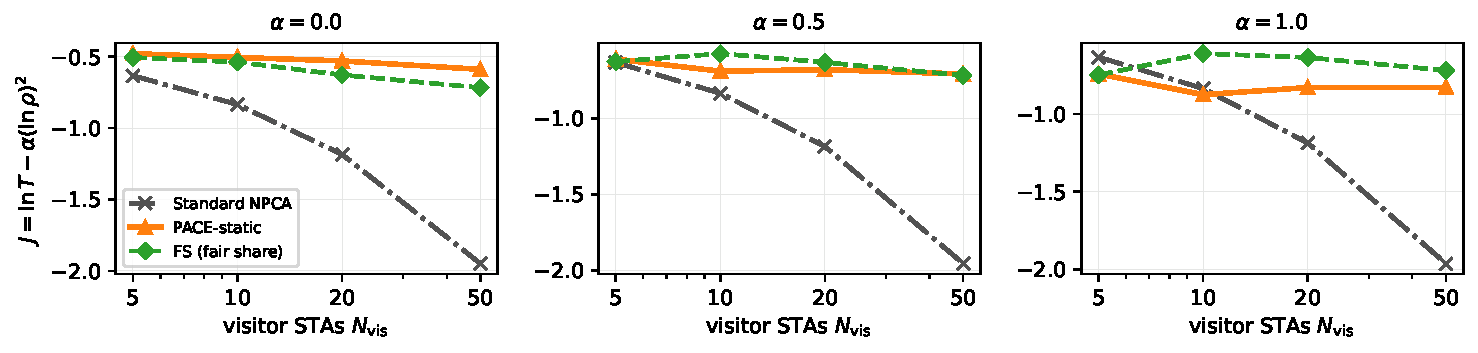
\includegraphics[width=0.92\textwidth]{figure/fig6-1.pdf}
        \caption{Basic access (no RTS/CTS).}
        \label{fig:objective_basic}
    \end{subfigure}
    \vspace{0.6em}

    \begin{subfigure}[b]{\textwidth}
        \centering
        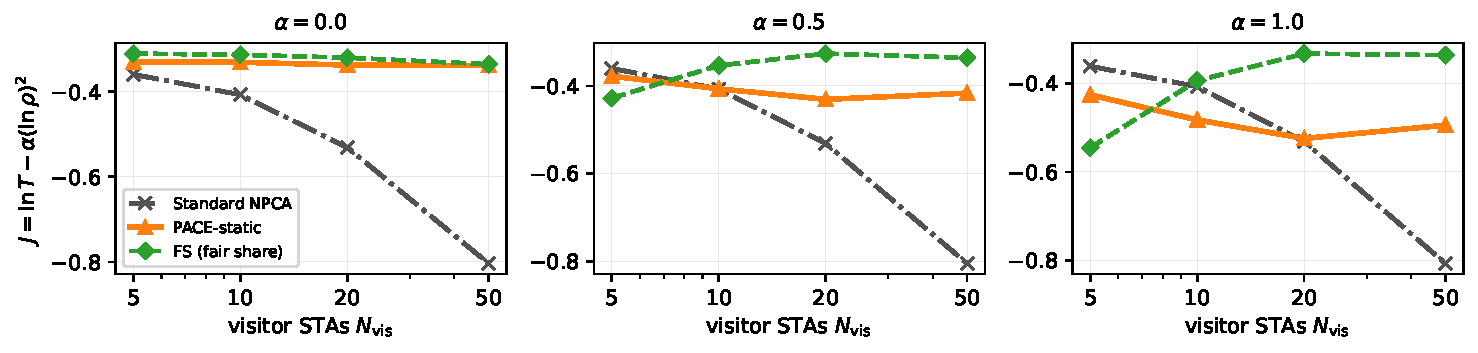
\includegraphics[width=0.92\textwidth]{figure/fig6-2.pdf}
        \caption{Mandatory RTS/CTS.}
        \label{fig:objective_rts}
    \end{subfigure}
    \caption{The combined objective of Eq.~\eqref{eq:objective} versus the
    number of visitor STAs, in the setting of Fig.~\ref{fig:why_pace}, for
    proportionality weights $\alpha\in\{0,\,0.5,\,1\}$.}
    \label{fig:objective}
\end{figure*}

Efficiency and proportionality can also be read on one axis.
Fig.~\ref{fig:objective} evaluates the objective of
Eq.~\eqref{eq:objective} across the visitor sweep for three settings of
the weight $\alpha$, which has no canonical value. At $\alpha=0$ the objective reduces to log airtime
and PACE sits at or above FS at every population. Raising $\alpha$
rewards proximity to the proportional line, which is FS's defining
property, so FS moves ahead by a growing margin, up to $0.26$ at
$\alpha=1$ under basic access, while PACE stays within about $0.1$ of
FS at the calibration weight $\alpha=0.5$. The one reordering appears
at $\Nvis=5$ under the full weight $\alpha=1$, where the standard
baseline scores best of the three; a lightly loaded channel loses
little airtime to its collisions and its share happens to sit near
proportional, whereas FS structurally over-serves ($\rho\approx1.6$)
and PACE under-serves. From $\Nvis=10$ onward, where contention
actually stresses the window, no weight changes the ranking. PACE and
FS remain close while the standard baseline trails by $0.3$ to $1.1$,
its collapse in $T$ dominating any proportionality credit. The
calibration weight $\alpha=0.5$ of Section~\ref{subsec:factor_scaling}
thus sits in the middle of the range in which the comparison is
insensitive to the weight. The comparison also flatters FS less than it
seems. FS is a genie policy that transmits at
$\tau^*(t)=1/|\mathcal{V}(t)|$ with per-slot knowledge of the viable
set, which presupposes not only the visitor population but the native
one and every contender's frame fit, whereas PACE reaches these scores
from local feedback alone, knowing neither $\Nvis$ nor $\Nnat$.
Near-parity with the genie at every weight is therefore the substantive
result of the figure.

\subsection{Impact of Visiting Duration}
\label{subsec:eval_duration}

\begin{figure}[t]
    \centering
    \begin{subfigure}[b]{\columnwidth}
        \centering
        
\includegraphics[width=\linewidth]{figure/fig3-1.pdf}
        \caption{Basic access (no RTS/CTS).}
        \label{fig:duration_basic}
    \end{subfigure}
    \vspace{0.6em}

    \begin{subfigure}[b]{\columnwidth}
        \centering
        
\includegraphics[width=\linewidth]{figure/fig3-2.pdf}
        \caption{Mandatory RTS/CTS.}
        \label{fig:duration_rts}
    \end{subfigure}
    \caption{Total useful airtime versus the visiting duration
    ($W_\mathrm{eff}$ of $100$--$1680$ slots, $0.9$--$15.1$~ms) for the
    standard procedure, PACE-static, PACE-dynamic, and FS, with
    $\Nvis=20$ visitor STAs and
    $\Nnat=10$ natives; all other parameters as in Table~\ref{tab:sim_params}.}
    \label{fig:duration}
\end{figure}

\begin{figure}[t]
    \centering
    \begin{subfigure}[b]{\columnwidth}
        \centering
        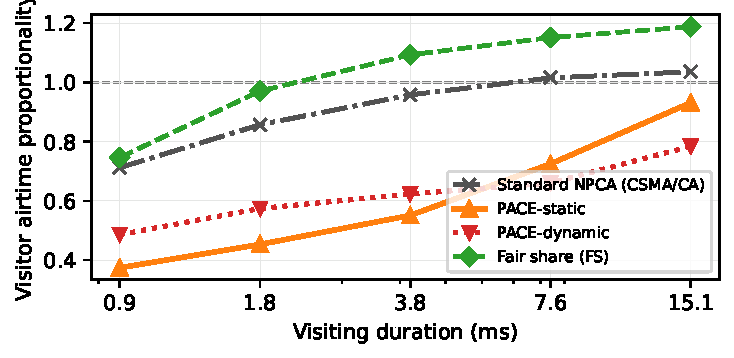
\includegraphics[width=\linewidth]{figure/fig3-3.pdf}
        \caption{Basic access (no RTS/CTS).}
        \label{fig:duration_rho_basic}
    \end{subfigure}
    \vspace{0.6em}

    \begin{subfigure}[b]{\columnwidth}
        \centering
        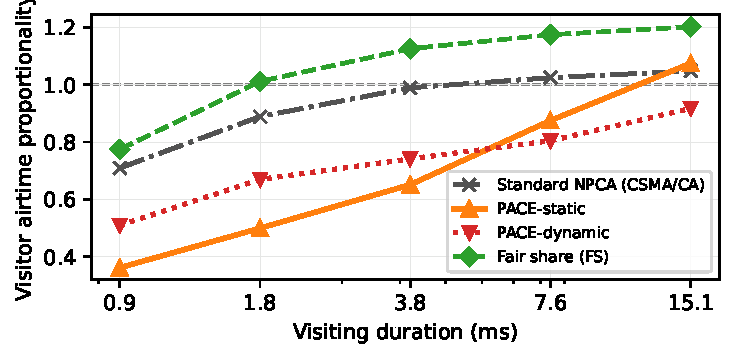
\includegraphics[width=\linewidth]{figure/fig3-4.pdf}
        \caption{Mandatory RTS/CTS.}
        \label{fig:duration_rho_rts}
    \end{subfigure}
    \caption{Visitor airtime proportionality $\rho$ versus the visiting
    duration, in the setting of Fig.~\ref{fig:duration}. The dashed line
    marks the proportional share $\rho=1$.}
    \label{fig:duration_rho}
\end{figure}

The window an NPCA visit receives is not a design choice but an
environmental one. It is the remaining duration of the OBSS transmission
that opened the opportunity, and it varies from sub-millisecond frames to
transmission opportunity (TXOP)-scale bursts. Fig.~\ref{fig:duration} therefore sweeps the visiting
duration from $0.9$ to $15.1$~ms, which corresponds to $1.6$ to $27$ mean
visitor frames, at
$\Nvis=20$ visitors and $\Nnat=10$ natives. This sweep is also where the
window scaling of Section~\ref{subsec:factor_scaling} faces its test, so
both variants appear, PACE-static with the fixed factor of
Table~\ref{tab:sim_params} and PACE-dynamic with the factor recomputed
from each visit's window, which falls from $2.76$ at the shortest window
to $1.28$ at the longest.

Under basic access, shown in Fig.~\ref{fig:duration_basic}, the standard
visitors hold the channel at $0.26$--$0.37$ across the sweep. However
long the visit lasts, $\mathrm{CW}_{\min}=16$ remains mismatched to the
$30$-station contention, and the synchronized collision cascades, each
charged a full frame length, consume a roughly constant fraction of
whatever window is available. Both PACE variants deliver $1.5\times$ to
$2.1\times$ the standard procedure, but they part at the ends of the
sweep. PACE-static declines from $0.61$ at $0.9$~ms to $0.50$ at
$15.1$~ms and slips below the FS line at the longest visits ($0.50$
against $0.53$), since a factor calibrated at the reference window keeps
raising the probability past the fair-share target once the visit lasts
long enough for the overshoot to accumulate. PACE-dynamic holds
$0.55$--$0.57$ and stays above FS at every duration.

Fig.~\ref{fig:duration_rho} shows what these totals cost in fairness.
PACE-static spans $\rho$ of $0.37$--$0.93$ under basic access and
$0.36$--$1.07$ under RTS/CTS, so the same fixed factor leaves the
visitors near a third of their proportional share in a $0.9$-ms visit
and pushes them past the proportional line in the longest protected
ones. Its higher short-window total in Fig.~\ref{fig:duration_basic} is
earned the same way, by under-serving its own visitors while the natives
fill the window. PACE-dynamic compresses the swing to $0.49$--$0.78$ and
$0.51$--$0.92$ and stays below proportionality at every duration. A
single coefficient thus errs in opposite directions at the two ends of
the range, too timid where the visit is short and too aggressive where
it is long, exactly the transient and fluctuation losses that
Section~\ref{subsec:factor_scaling} balances, and the
inverse-square-root rule corrects both without any additional signaling.

Under mandatory RTS/CTS, shown in Fig.~\ref{fig:duration_rts}, the
airtime differences narrow because the handshake caps the collision
cost. The standard visitors stay $8$--$18\%$ below PACE-static
throughout, at $0.59$--$0.66$, and the margin does not close as the
window grows, since the losses caused by the backoff recur under
saturation, where every completed exchange re-enters contention with a
reset contention window. The two PACE variants track FS closely and
nearly coincide in total airtime, with the long-window edge going to
PACE-dynamic ($0.73$ against $0.72$, FS at $0.75$), so under this access
mode the value of the window scaling lies less in airtime than in
Fig.~\ref{fig:duration_rho_rts}, where PACE-dynamic keeps the visitors
below the proportional line that the fixed factor crosses. At short
durations both variants leave the visitors a smaller share of the window
than the standard visitors do, the one-probe budget
$\tau_0=1/W_\mathrm{eff}$ leaves the feedback little room to ramp, but
the composition is the fair one. The slots PACE declines to contest
carry native traffic, keeping the total above the standard procedure
at every duration.

\subsection{Tracking the Time-Varying Fair-Share Target}
\label{subsec:eval_tracking}

\begin{figure}[t]
    \centering
    \begin{subfigure}[b]{\columnwidth}
        \centering
        
\includegraphics[width=\linewidth]{figure/fig4-1.pdf}
        \caption{Basic access (no RTS/CTS).}
        \label{fig:tracking_basic}
    \end{subfigure}
    \vspace{0.6em}

    \begin{subfigure}[b]{\columnwidth}
        \centering
        
\includegraphics[width=\linewidth]{figure/fig4-2.pdf}
        \caption{Mandatory RTS/CTS.}
        \label{fig:tracking_rts}
    \end{subfigure}
    \caption{Within-visit transmission dynamics in the reference setting
    of Fig.~\ref{fig:why_pace} ($\Nvis=20$, $\Nnat=10$,
    $W_\mathrm{eff}=420$ slots, $3.78$~ms). The analytic FS target
    $\tau^*(t)=1/|\mathcal{V}(t)|$ and the measured per-slot
    transmission rate of viable visitors under PACE-static,
    PACE-dynamic, and the standard procedure, averaged over $500$
    visits.}
    \label{fig:tracking}
\end{figure}

The aggregate results of Sections~\ref{subsec:eval_whypace}%
--\ref{subsec:eval_duration} follow from the within-visit transmission
behavior of each scheme, which Fig.~\ref{fig:tracking} reports. Since the standard visitor holds no per-slot probability, we
plot for every scheme the same model-free quantity, the measured
fraction of viable visitors transmitting in each slot, against the
analytic FS target. The target $\tau^*(t)$ stays near $1/(\Nvis{+}\Nnat)=1/30$
for most of the visit and then rises steeply in the final slots, as
PPDU-aware self-exclusion drains the viable
set. 

The standard-compliant visitor enters at $1/\mathrm{CW}_{\min}=1/16$,
roughly twice the target, and its measured rate then remains near the
target even though the scheme does not estimate it. The aggregate rate, however, conceals the
failure mechanism. The countdown is deterministic and freezes during every busy
period, so multiple backoff counters expire together once the medium
becomes idle, and attempts at the same average rate collide far more
often than independent ones, $84$--$86\%$ of standard-visitor transmissions
collide, against $59$--$60\%$ for FS at a comparable rate
(Table~\ref{tab:attempts}). The aggregate rate is moreover
sustained by the few STAs that happen to draw short backoffs, while
each collision doubles the contention windows of the remaining STAs
without an in-visit reset, so the airtime distribution across visitors
becomes increasingly uneven although the aggregate rate is maintained.

PACE requires neither knowledge of the target nor favorable backoff
draws. It enters at
$\tau_0=1/W_\mathrm{eff}$, deliberately below the target, and the
idle-driven multiplicative increase together with solo-copy propagation
raises the measured rate toward the target from below over the
course of the visit; being genuinely probabilistic, its attempts
stay uncorrelated, and they collide at essentially the rate of the FS
reference (Table~\ref{tab:attempts}). Approaching the
target from below is the safe direction established in
Section~\ref{subsec:init}. An under-aggressive probability costs a few
idle slots, which the feedback recovers quickly, whereas over-aggressive
or synchronized attempts consume the window in full-frame collisions
that no subsequent adaptation can recover. The same qualitative picture holds
in both access modes; under RTS/CTS the convergence is tighter because
each corrective feedback event costs at most the constant
$L_\mathrm{col}$ rather than a full frame.

\begin{figure*}[t]
    \centering
    \begin{subfigure}[b]{\textwidth}
        \centering
        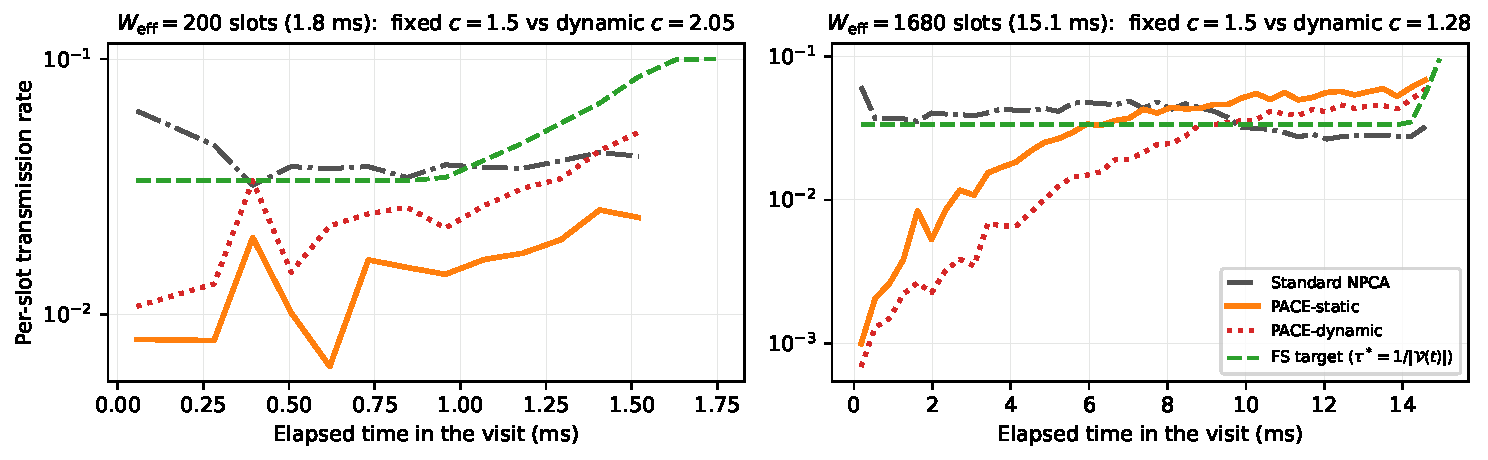
\includegraphics[width=0.92\textwidth]{figure/fig4-3.pdf}
        \caption{Basic access (no RTS/CTS).}
        \label{fig:tracking_windows_basic}
    \end{subfigure}
    \vspace{0.6em}

    \begin{subfigure}[b]{\textwidth}
        \centering
        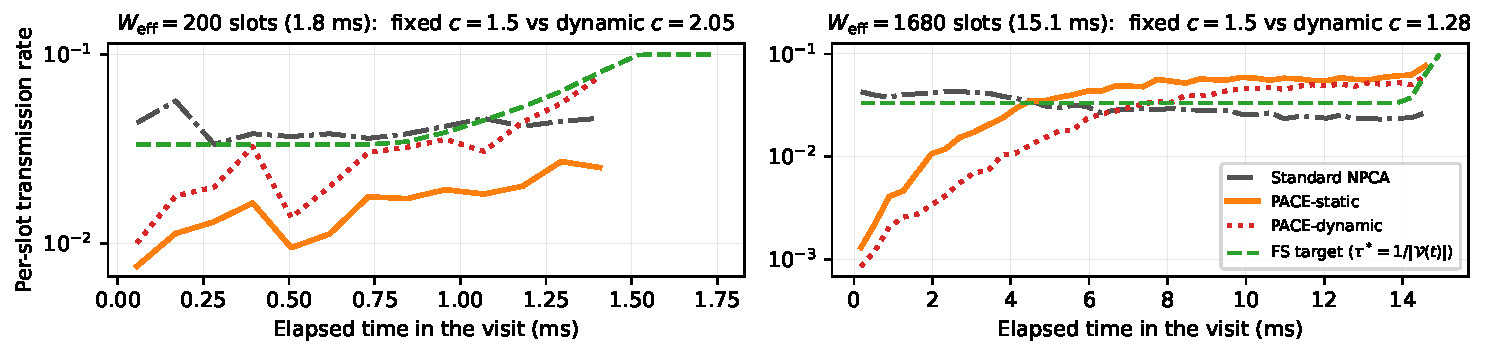
\includegraphics[width=0.92\textwidth]{figure/fig4-4.pdf}
        \caption{Mandatory RTS/CTS.}
        \label{fig:tracking_windows_rts}
    \end{subfigure}
    \caption{Within-visit transmission dynamics at the two ends of the
    window sweep of Fig.~\ref{fig:duration} ($W_\mathrm{eff}$ of $100$
    and $1680$ slots, $0.9$ and $15.1$~ms, $\Nvis=20$, $\Nnat=10$).
    PACE-static keeps the fixed factor $c=1.5$ at both windows, while
    PACE-dynamic recomputes it per visit, $c=2.76$ at the short window
    and $c=1.28$ at the long one.}
    \label{fig:tracking_windows}
\end{figure*}

Fig.~\ref{fig:tracking} is drawn at the reference window, where the
factor PACE-dynamic computes, $1.64$, differs little from the fixed
$1.5$ and the two variants trace nearly the same path. The distinction
appears at the ends of the window sweep, which
Fig.~\ref{fig:tracking_windows} redraws. In a $0.9$-ms visit the fixed
factor never lifts the rate to the target before the window closes,
which is the transient loss of Section~\ref{subsec:factor_scaling} made
visible, whereas the per-visit factor of $2.76$ arrives with slots to
spare. In a $15.1$-ms visit the same fixed factor crosses the target
partway through and keeps the rate above it for the remainder, the
accumulated fluctuation loss, while the factor of $1.28$ settles onto
the target and stays there. The two failure modes are symmetric, and
correcting them at the trajectory level is what produces the airtime
crossing and the compressed fairness swing of
Figs.~\ref{fig:duration} and~\ref{fig:duration_rho}.

\begin{table}[t]
\centering
\caption{Per-Attempt Outcome of Visitor Transmissions\\(setting of Fig.~\ref{fig:tracking}, steady state)}
\label{tab:attempts}
\begin{tabular}{llccc}
\hline
\textbf{Access} & \textbf{Scheme} & \textbf{Succ.} & \textbf{Coll.} & \textbf{Att./frame} \\
\hline
basic   & Standard & $16\%$ & $84\%$ & $6.5$ \\
        & PACE-static   & $44\%$ & $56\%$ & $2.3$ \\
        & PACE-dynamic  & $40\%$ & $60\%$ & $2.5$ \\
        & FS            & $40\%$ & $60\%$ & $2.5$ \\
\hline
RTS/CTS & Standard & $14\%$ & $86\%$ & $7.3$ \\
        & PACE-static   & $40\%$ & $60\%$ & $2.5$ \\
        & PACE-dynamic  & $35\%$ & $65\%$ & $2.8$ \\
        & FS            & $41\%$ & $59\%$ & $2.4$ \\
\hline
\end{tabular}
\end{table}

Table~\ref{tab:attempts} classifies every visitor transmission attempt
in the setting of Fig.~\ref{fig:tracking} and summarizes the
contention efficiency of each scheme. Only $14$--$16\%$ of the
standard visitors' transmission attempts succeed; the rest are
synchronized collisions, so the standard procedure transmits six to
seven times to deliver a single frame. PACE completes $40$--$44\%$ of
its attempts and delivers a frame in about two and a half
transmissions, which is essentially the per-attempt outcome of FS
itself; PACE-dynamic, whose per-visit factor at this window is the
slightly more aggressive $1.64$, sits a few points lower at
$35$--$40\%$ while delivering the same airtime. A high success ratio alone could be achieved by transmitting
rarely, so the result is meaningful only in combination with
Fig.~\ref{fig:why_pace}. PACE attains the highest total airtime of the
three schemes while spending about the same number of transmissions
per delivered frame as the fair-share reference, whereas the standard procedure
retransmits the most and delivers the least; the scheme does not beat
the fair operating point, it reaches it without being told where it
is.

\subsection{Ablation Study}
\label{subsec:eval_ablation}

\begin{figure}[t]
    \centering
    \begin{subfigure}[b]{\columnwidth}
        \centering
        
\includegraphics[width=\linewidth]{figure/fig5-1.pdf}
        \caption{Basic access (no RTS/CTS).}
        \label{fig:ablation_basic}
    \end{subfigure}
    \vspace{0.6em}

    \begin{subfigure}[b]{\columnwidth}
        \centering
        
\includegraphics[width=\linewidth]{figure/fig5-2.pdf}
        \caption{Mandatory RTS/CTS.}
        \label{fig:ablation_rts}
    \end{subfigure}
    \caption{Ablation study in the setting of Fig.~\ref{fig:why_pace}:
    total useful airtime for full PACE, PACE without PPDU-aware
    self-exclusion, PACE without the one-probe initialization, and the standard-compliant baseline.}
    \label{fig:ablation}
\end{figure}

PACE adds two mechanisms to the MIMD adaptation rule, the one-probe
initialization $\tau_0=1/W_\mathrm{eff}$ of Phase~(a) and the PPDU-aware
self-exclusion of Phase~(b). Fig.~\ref{fig:ablation} removes each in
turn in the setting of Fig.~\ref{fig:why_pace}. The initialization
determines the behavior at the beginning of the visit and
self-exclusion determines the behavior at its end. The third design
choice, the adaptation step of Section~\ref{subsec:factor_scaling},
distinguishes itself only when the window varies, so its ablation is
the static-to-dynamic comparison of
Section~\ref{subsec:eval_duration}; at the reference window of this
experiment the two variants nearly coincide, and the runs here use
PACE-static.

Replacing the initialization with the knowledge-free choice
$\tau_0\sim\mathcal{U}(0,1)$, a natural prior when no population
estimate is available, reduces the total airtime under basic access to
$0.17$--$0.03$, below even the standard baseline at every population.
The visit begins with a large number of simultaneous transmissions,
each collision is charged the longest colliding frame, and the
multiplicative decrease is too slow to bring $\tau$ to the operating
point of order $10^{-2}$ before the window ends. Under RTS/CTS the
totals of $0.42$--$0.15$ also remain below the standard baseline,
because a second failure mechanism operates in addition to the initial
collisions. Visitors drawn near $\tau\approx 1$ transmit in almost
every slot, so solo successes, the events that propagate a common
operating point through the copy rule of~\eqref{eq:mimd}, rarely
occur, and the population cannot converge to a lower $\tau$. The same experiment shows a fairness deficit as well. At $\Nvis=5$
under RTS/CTS the visitors occupy most of the useful airtime while the
ten natives obtain almost none. A probabilistic access scheme without a
deadline-scaled initialization therefore performs worse than the
backoff procedure it replaces, so the conservative initialization is a
precondition for PACE rather than an optimization.

Removing self-exclusion causes a smaller but systematic loss that
grows with the visitor population. Total airtime decreases by
$3$--$7\%$ across the sweep under both access modes, at $\Nvis=50$
from $0.556$ to $0.520$ under basic access and from $0.714$ to
$0.672$ under RTS/CTS. Without Phase~(b) a visitor whose frame no
longer fits keeps contending and raises the collision rate observed by
the STAs that can still succeed, and when it does obtain the channel
it starts a transmission that the NPCA timer terminates, so the final
part of the window is lost. Self-exclusion returns both losses to the
remaining viable STAs. The ablated variant still exceeds the standard
baseline by a wide margin, which indicates that the MIMD adaptation is
the dominant mechanism and that self-exclusion prevents its gains from
degrading near the deadline.

\section{Conclusion}
\label{sec:conclusion}

This paper presented PACE, a probabilistic adaptive contention control
scheme for non-primary channel access in IEEE~802.11bn. Inside the
bounded NPCA visit the fair operating point
$\tau^*(t)=1/|\mathcal{V}(t)|$ rises toward the deadline, whereas BEB
lowers its attempt rate after every collision and loses the window to
synchronized collisions and frozen counters. PACE replaces the backoff
countdown with a per-slot transmission probability governed by three
local rules, namely the one-probe initialization
$\tau_0=1/W_\mathrm{eff}$, PPDU-aware self-exclusion, and MIMD
adaptation with solo-copy consensus, and requires neither central
coordination nor knowledge of the contending population.

Simulations under IEEE~802.11 timing with native DCF stations showed
that PACE keeps the total useful airtime within $3\%$ of a genie-aided
fair-share reference under RTS/CTS-protected access, exceeds the
standard-compliant baseline by up to $61\%$ there and by up to
$4.1\times$ under basic access, and holds the visitors' airtime at or
below their population-proportional share across visit durations of
one to fifteen milliseconds. Each delivered frame costs a quarter of
the transmission attempts that the standard procedure requires. An
ablation study confirmed that both the deadline-scaled initialization
and the self-exclusion rule are necessary for these gains.

Future work includes a cost-aware decrease factor that weights
collisions by their observed channel occupancy, partial-overlap
topologies with spatial reuse, TXOP aggregation within a visit, and
warm-starting $\tau$ across repeated visits to shorten the ramp-up in
sub-millisecond windows.

\bibliographystyle{IEEEtran}
\bibliography{pace}

\end{document}
